%----------------------------------------------------------------------------------------
%	PACKAGES AND OTHER DOCUMENT CONFIGURATIONS
%----------------------------------------------------------------------------------------

\documentclass[12pt]{article}
\usepackage{graphicx}
\usepackage[utf8]{inputenc}  
\usepackage[T1]{fontenc} 
\usepackage[top=2cm,bottom=2cm,left=1.3cm,right=1cm,asymmetric]{geometry}

\usepackage{amsfonts}
\usepackage{fancyhdr}
\usepackage{array,multirow,makecell}
\usepackage{amsmath}

\usepackage{cancel}
\usepackage{subfig}
\usepackage{wrapfig}
\usepackage[table]{xcolor}

\newcommand\independent{\protect\mathpalette{\protect\independenT}{\perp}}
\def\independenT#1#2{\mathrel{\rlap{$#1#2$}\mkern2mu{#1#2}}}

\setcellgapes{1pt}
\makegapedcells
\newcolumntype{R}[1]{>{\raggedleft\arraybackslash }b{#1}}
\newcolumntype{L}[1]{>{\raggedright\arraybackslash }b{#1}}
\newcolumntype{C}[1]{>{\centering\arraybackslash }b{#1}}

\pagestyle{fancy}
\renewcommand{\footrulewidth}{1pt}
\fancyhead[R]{\textit{Master MVA : Graphical models}}
\fancyfoot[L]{\textit{}}
%\usepackage{unicode-math}
%\setmathfont{XITS Math}
%\setmathfont[version=setB,StylisticSet=1]{XITS Math}


%\geometry{hmargin=1.5cm,vmargin=2cm}   

\begin{document}


\section*{Sammy Khalife \& Matias Tailanian}
\subsubsection*{29/10/2014}
\subsubsection*{Assignment 2}
\section*{1 Distributions factorizing in a graph} 
\subsection*{a.}
- Given the definition of $p \in L(G)$, we have for any x :
\begin{eqnarray*}
p(x) & = & \prod_{k=1}^{n}p(x_{k}|x_{\pi_{k}})\\
& = &  \prod \limits^n_{\substack{k=1 \\ k \neq i k \neq j} }p(x_{k}|x_{\pi_{k}}) \; p(x_{i}|x_{\pi_{i}})p(x_{j}|x_{\pi_{i}},x_{i})
\end{eqnarray*}
Since by assumption, $\pi_{j}=\pi_{i} \cup {i}$: $p(x_j|x_{\pi_j})=p(x_j|x_{\pi_{i\cup i}})=p(x_j|x_{\pi_i},x_i)$.~\\
Thanks to the Bayes formula applied to $p(x_{j}|x_{\pi_{i}}, x_{i})$ :
\begin{eqnarray*}
p(x) & = & \prod \limits_{\substack{k=1 \\ k \neq i k \neq j} } p(x_{k}|x_{\pi_{k}})        
\cancel {p(x_{i}|x_{\pi_{i}})}
p(x_{i}|x_{\pi_{i}},x_{j})\frac{p(x_{j}|x_{\pi_{i}})}{\cancel{p(x_{i}|x_{\pi_{i}})}}\\
& = &  \prod \limits_{\substack{k=1 \\ k \neq i k \neq j} } p(x_{k}|x_{\pi_{k}})p(x_{i}|x_{\pi_{i}},x_{j})p(x_{j}|x_{\pi_{i}})
\end{eqnarray*}
This last equality is saying that $p$ is factorizing in $G^{'}=(V,E^{'})$, with $E^{'} = (E \setminus \{ i \mapsto j \}\cup\{j\mapsto i\})$. ~\\
Then $L(G) \subset L(G')$.~\\
By going back in the equalities, we actually have $L(G^{'}) \subset L(G)$.
Hence, $L(G)=L(G^{'})$.
~\\
~\\
- As $G$ is a directed tree, it's also a \emph{graph}, so $p(x)$ factorizes in $G$:
$$p(x) = \prod^n_{i=1}p(x_i|x_{\pi_i})$$
As $G$ is a directed tree with no \emph{v-structures}, it has the same quantity of \emph{edges} as \emph{clicks}: $n-1$. Furthermore each click has two elements, i.e. sets parent-children. Dividing and multiplying the previous expression by $n-1$, and defining $\psi_{c}(x_{c}) = (n-1)^{\frac{1}{n}}f(x_c,x_{\pi_c})$ (without ambiguity because there is only one node having no parents in the clique) and $Z=n-1$ (the number of clicks), we obtain:
$$p(x) = \frac{1}{Z}\prod_{c\in \mathcal{C}}\psi_c(x_c)$$
where $\mathcal{C}$ is the set of clicks of $G$. This expression corresponds to a factorization in the symetrized graph $G^\prime$ of $G$, which has $Z=n-1$ clicks of cardinal $2$, $\{x_k, x_{\pi_k}\}$, proving: $\mathcal{L}(G)\subseteq \mathcal{L}(G^\prime)$.
~\\
~\\
In the other hand, as $E^\prime \subseteq E$, as a general result on graphical models : $\mathcal{L}(G^\prime)\subseteq \mathcal{L}(G)$.
Finally, $$\boxed{\mathcal{L}(G) = \mathcal{L}(G^\prime)}$$
%TODO: doubt. (n-1) inside the prod?

\subsection*{b.}
First we know that for any directed graph $G$, and its symmetrized graphed $G'$, we always have $L(G)\subset L(G')$.~\\
Then, we just have to discuss the case $L(G') \subset  L(G)$.~\\
~\\
For a 2 nodes-graph, if there is an edge. we always have for p $\in L(G'), p(x)=p(x2|x1)p(x1)$, this corresponds to a trival directed graph. If there is no edge, then the directed graph with no edge corresponds to the same factorization of p in the symmetrized graph.~\\
~\\
For a 3 nodes-graph :~\\
- No-edges graph : all the nodes are independant, then the factorization is the same in the directed graph with no no edges.~\\
- One-edge graph : there is only one clique containing more than one node (2 nodes)  in the undirected graph, with a factorization :~\\
$$p(x) = [\prod^n \limits_{\substack{i=1 \\ i \neq i_{0} i \neq {i_{1}} } }\psi_{i}(x_i)] \: \psi_{i_{0},i_{1}}(x_{i_{0}},x_{i_{1}})$$
This corresponds to a factorization in a directed graph with the same edge oriented in any direction.~\\
- 2 edges-graph : Then, the graph is an undirected tree with no v-structures, and we use the result of 1.b to have $L(G)=L(G')$.~\\
~\\
Let's consider a 4 nodes graph like the following :~\\
% figure of counter exemple

%$$p(x)=\psi_{1}(x_{1},x_{2})\psi_{2}(x_{2}, x_{3}) \psi_{3}(x_{3}, x_{4})\psi_{4}(x_{4}, x_{1})$$

~\\
A directed graph should have the same edges, otherwise some independances would be erased or added (intuitive statement).
Moreover, there must be a v-structure, otherwise the directed graph would be cyclic and not be a DAG. Let's suppose this v-structure is on the node 1.
Then, 2 is not independant of 4 given (1,3) since there is a v-structure in (1,3), whereas in the symmetrized graph, 2 is independant of 4 given (1,3).  
This shows that p is in L(G) but not in L(G').~\\
The smallest undirected graph G' such that there is no directed graph G with L(G')=L(G) contains 4 nodes.


\section*{2 d-separation}
\subsection*{a.}
Let us denote $\mathbf{G_M}=(E, V_{M})$ the moral graph of $\mathbf{G}$, and let us suppose that S separates A and B in $\mathbf{G_M}$.~\\
~\\
Then, every chain going from A to B goes through a node in S, in $\mathbf{G_M}$ and in $\mathbf{G}$ . ~\\
Let c be a chain in $\mathbf{G}$, then it goes through at least one node in S.~\\
-If there is at least 2 nodes of the chain that are in S, there exists a non v-structure in S (indeed, two consecutive nodes cannot form both a v-structure), then the chain is blocked.~\\
-Otherwise, if the chain contains only one node d in S, with $d_{-} \in A$ and $d_{+} \in B$, we show that $(d_{-},,d,d,_{+})$ cannot be a v-structure. If it was, then $(d_{-}, d_{+}) \in V_{M}$, and would be a chain in the moral graph that does not go through S : this is a contradiction.~\\
A and B are d-separated by S in $\mathbf{G}$.


\subsection*{b.}
This property of transitivity for d-separation is false. 2 counterexamples are shown in the figure below.
\begin{figure} [h!]
\centering
  \subfloat[Simple DAG : T separates A and S but contains a v-structure in a chain going from A to B]{\label{fig:dagSimple} 
  		\includegraphics[width=.4\textwidth]{./pics/dagSimple.png}} \hfill 
  \subfloat[Complex DAG]{\label{fig:dagComplex} 
  		\includegraphics[width=.5\textwidth]{./pics/dagComplex.png}} \\
  \caption{Counterexamples}
  \label{fig:ex2_dags}
\end{figure}

\subsection*{c.}
\begin{wrapfigure}{r}{0.4\textwidth}
	\vspace{-20pt}
	\begin{center}
		\includegraphics[width=0.3\textwidth]{./pics/ex2c.png}
	\end{center}
	\vspace{-20pt}
	\caption{Graph $G$}
	\label{fig:ex2c}
\end{wrapfigure}
Given the graph shown in Figure \ref{fig:ex2c}, we consider the following statements:
\begin{enumerate}
	\item $X_{\{1,2\}}\independent X_4|X_3$
	\item $X_{\{1,2\}}\independent X_4|X_5$
	\item $X_1\independent X_6|X_{\{2,4,7\}}$
\end{enumerate}
1-TRUE.~\\
First we can see that $A=\{1,2\}$ and $B=\{4\}$ are d-separated by $C=\{3\}$. Indeed the chains going from A to B are exactly $(1,8,4)$ and $(2,8,4)$. Given that $\{8\}$ is a v-structure which is not in C, and C contains no descendants of $\{8\}$, these chains are locked in $\{8\}$, the statement 1 is true thanks to the Global Markov property.~\\
~\\
2-FALSE.
We can see that $A=\{1,2\}$ and $B=\{4\}$ are not d-separated by $C=\{5\}$, since the only chain going from A to B contains $\{7\}$ which is not a V-structure, and is not in C.~\\
~\\
3-TRUE.~\\
We show that $A=\{1\}$ and $B=\{6\}$ are d-separated by $C=\{2,4,7\}$. Indeed, the only chain going from A to B is $\{1,8,7,6\}$, and this chain is blocked in 7 since $7\in C$ and $\{8, 7, 6\}$ is not a v-structure. Given $p\in L(G)$, it verifies the Global Markov property, i.e $X_{A} \bot X_{B} | X_{C}$. The statement is true.~\\

\section*{Implementation - Gaussian Mixtures}
\subsection*{a.}
\begin{figure}[h!]
	\centering 
	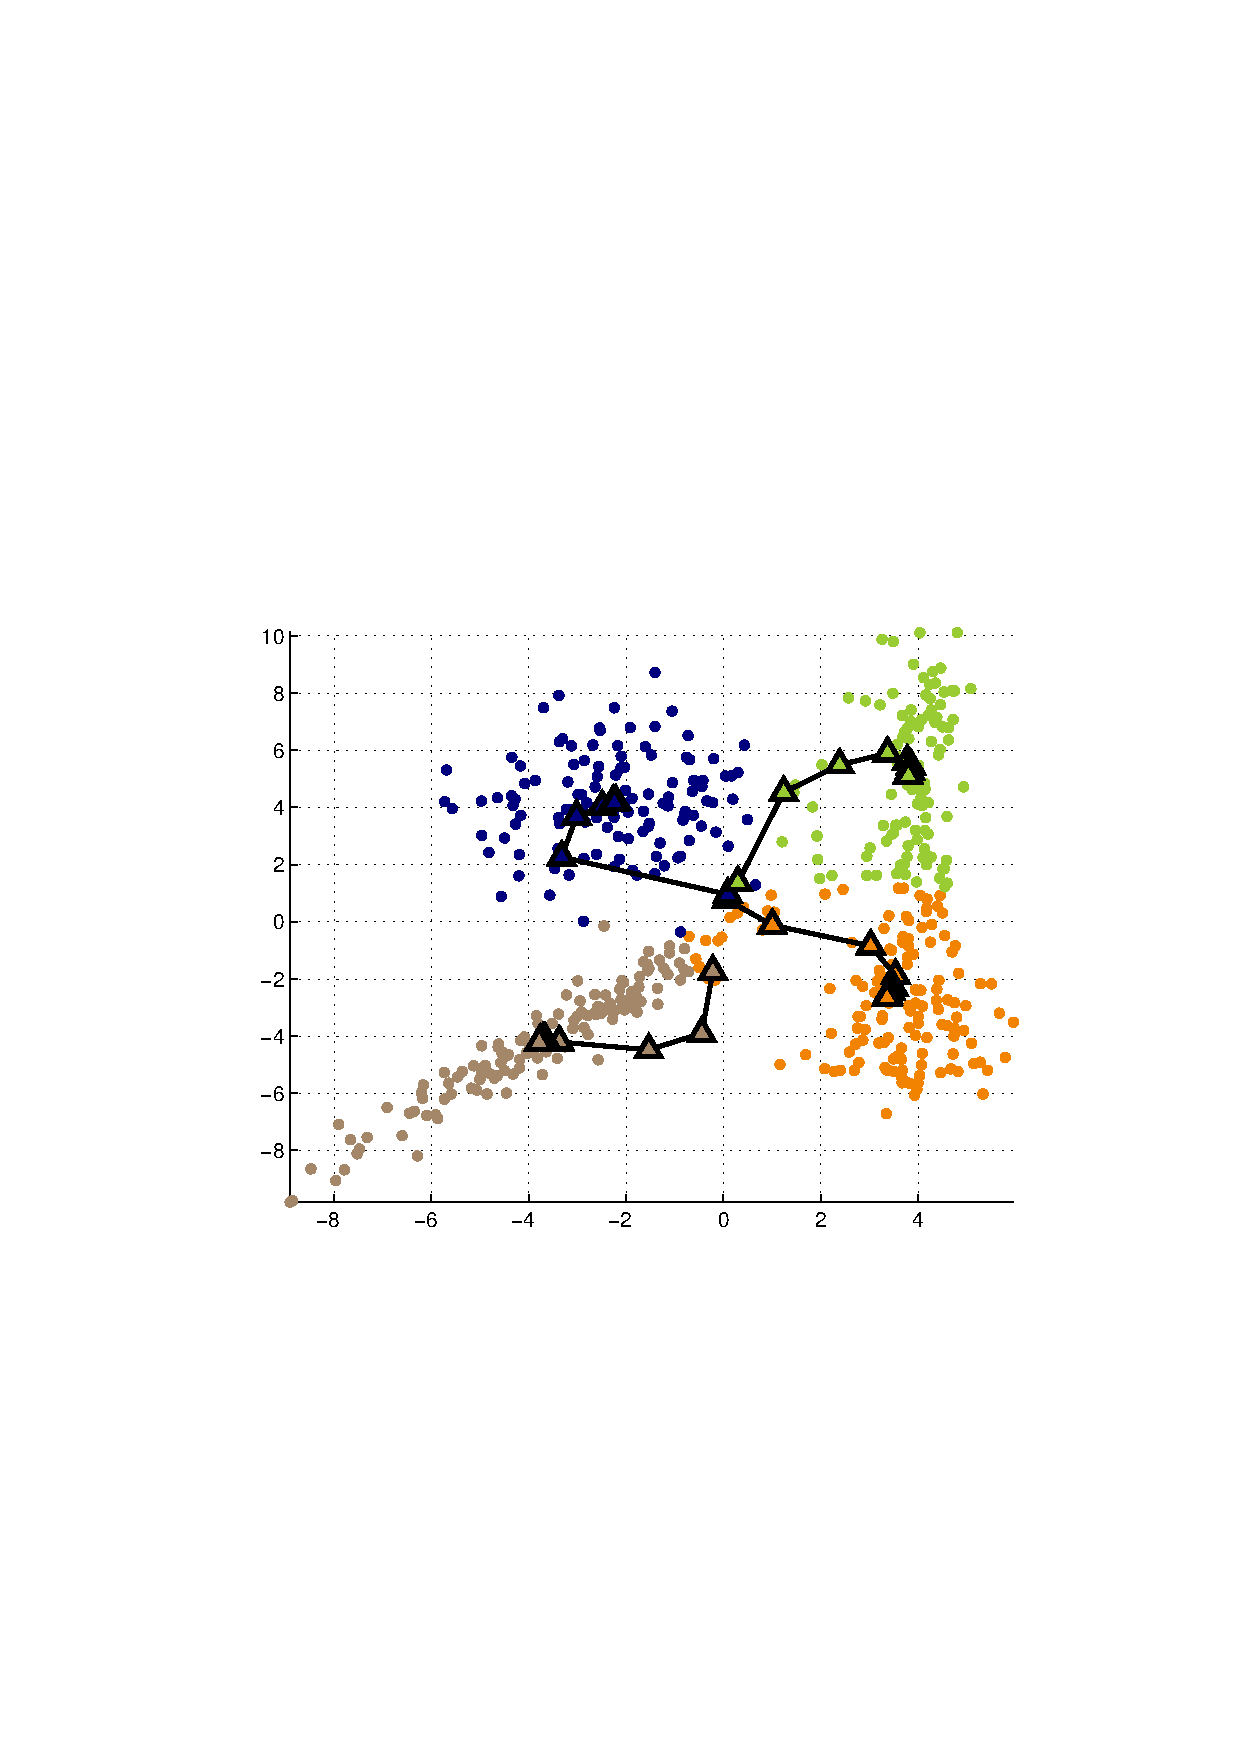
\includegraphics[width=.8\textwidth]{./pics/3a.pdf}
	\caption{K-Means algorithm output}
	\label{fig:3a}
\end{figure}
~\\
The distorsion of the clustering is invariant to the random initialization of the means, and equal to  3.2406e+03.~\\

\subsection*{b.}
Under the assumption that $\Sigma_{j} = \sigma Id$, the $\Sigma$ term in the log-likelyhood is just ~\\
$N log(\frac{1}{\sigma^{K}})-\frac{1}{2\sigma^{2}} \sum \limits_{i=1}^N ||x_{i}-\mu_{j}||^{2}$, then maximizing with respect to $\sigma$ yields :~\\
$\sigma=\sqrt{\frac{1}{2KN}\sum \limits_{i,j} ||x_{i}-\mu_{j}||^2}$~\\
For the other parameters $\Pi$ and $\mu$, the updating formulas are the same as in the general case for $\Sigma$
\begin{figure}[h!]
	\centering 
	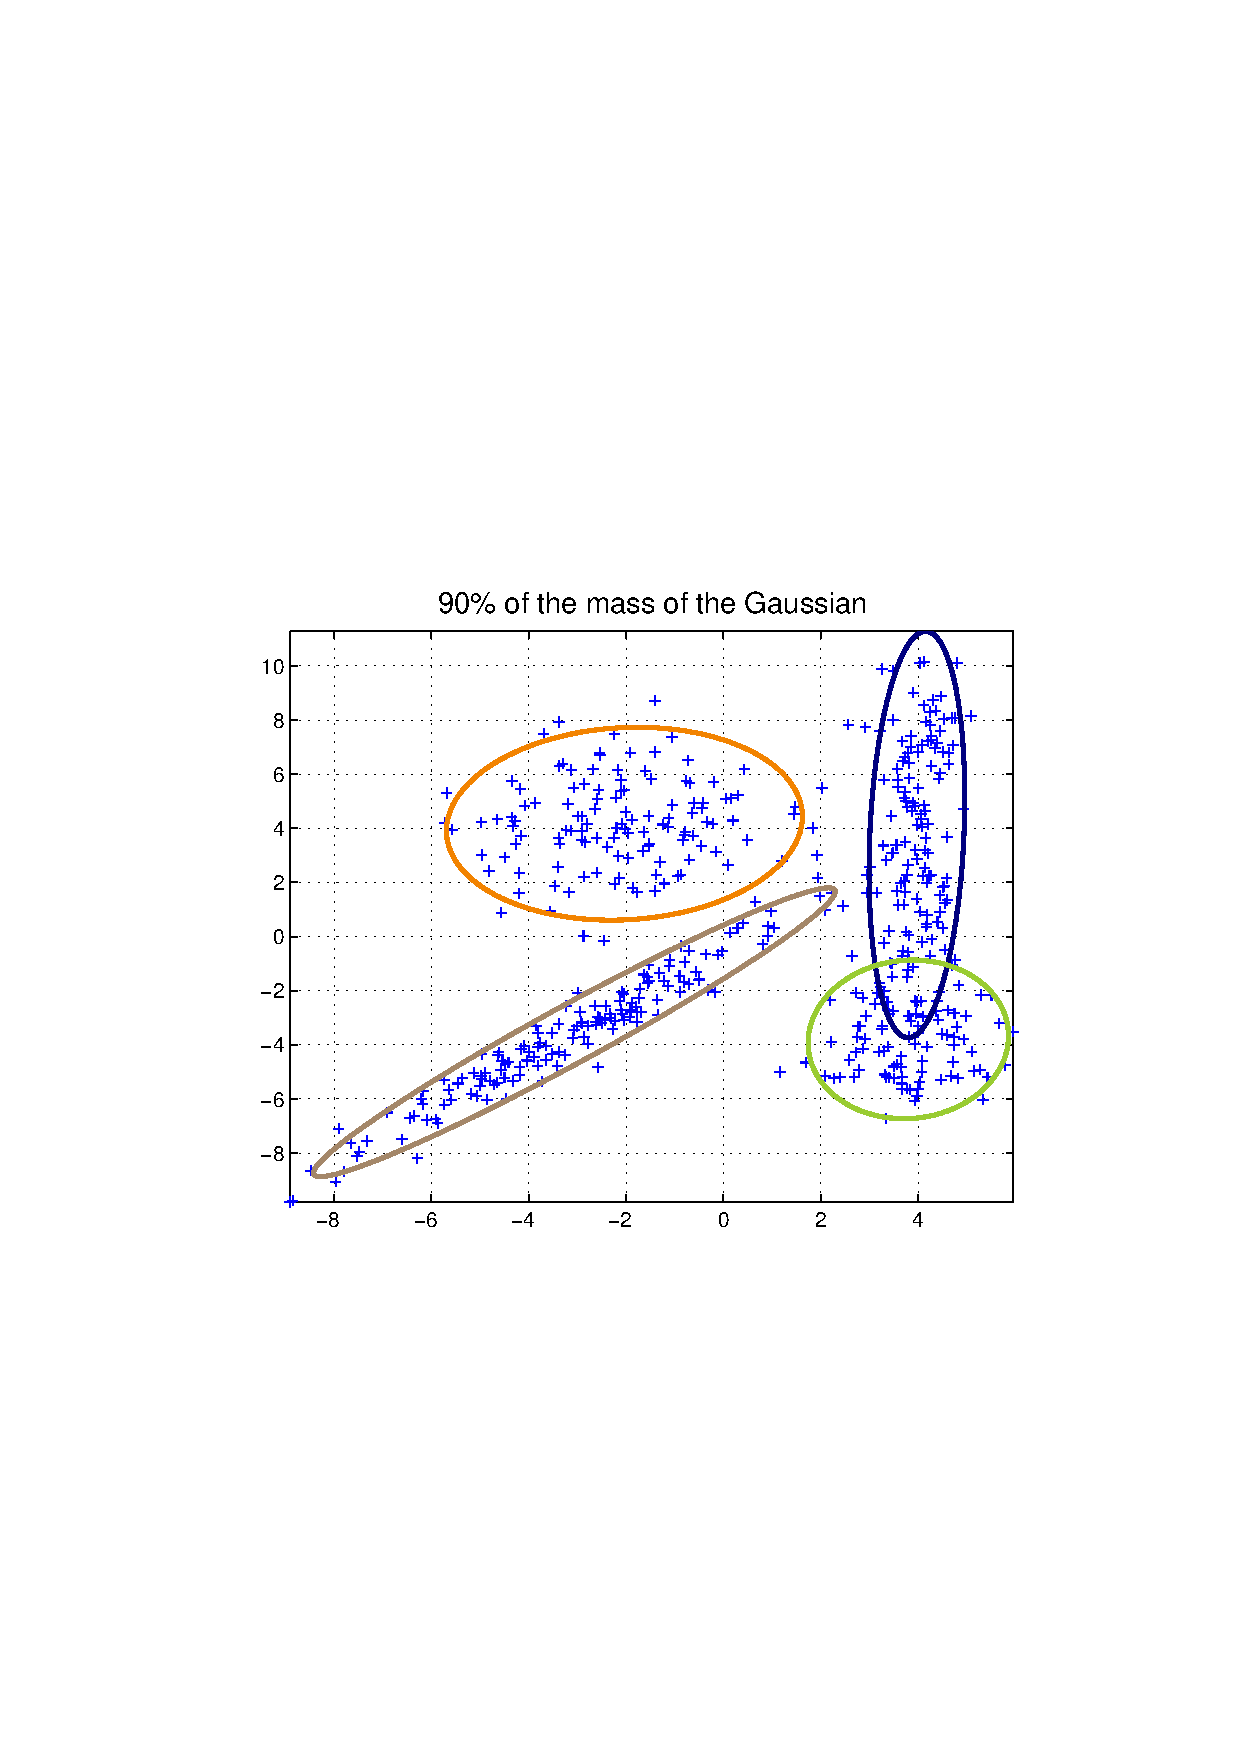
\includegraphics[width=.8\textwidth]{./pics/3b.pdf}
	\caption{Expectation maximization: 90\% mass of the Gaussian}
	\label{fig:3b}
\end{figure}

\subsection*{c}
In the case of general form matrix $\Sigma$, we have the classical updating formulas for the EM algorithm.
<<<<<<< HEAD
Values of the log-likelyhood
=======
\begin{figure}[h!]
	\centering 
	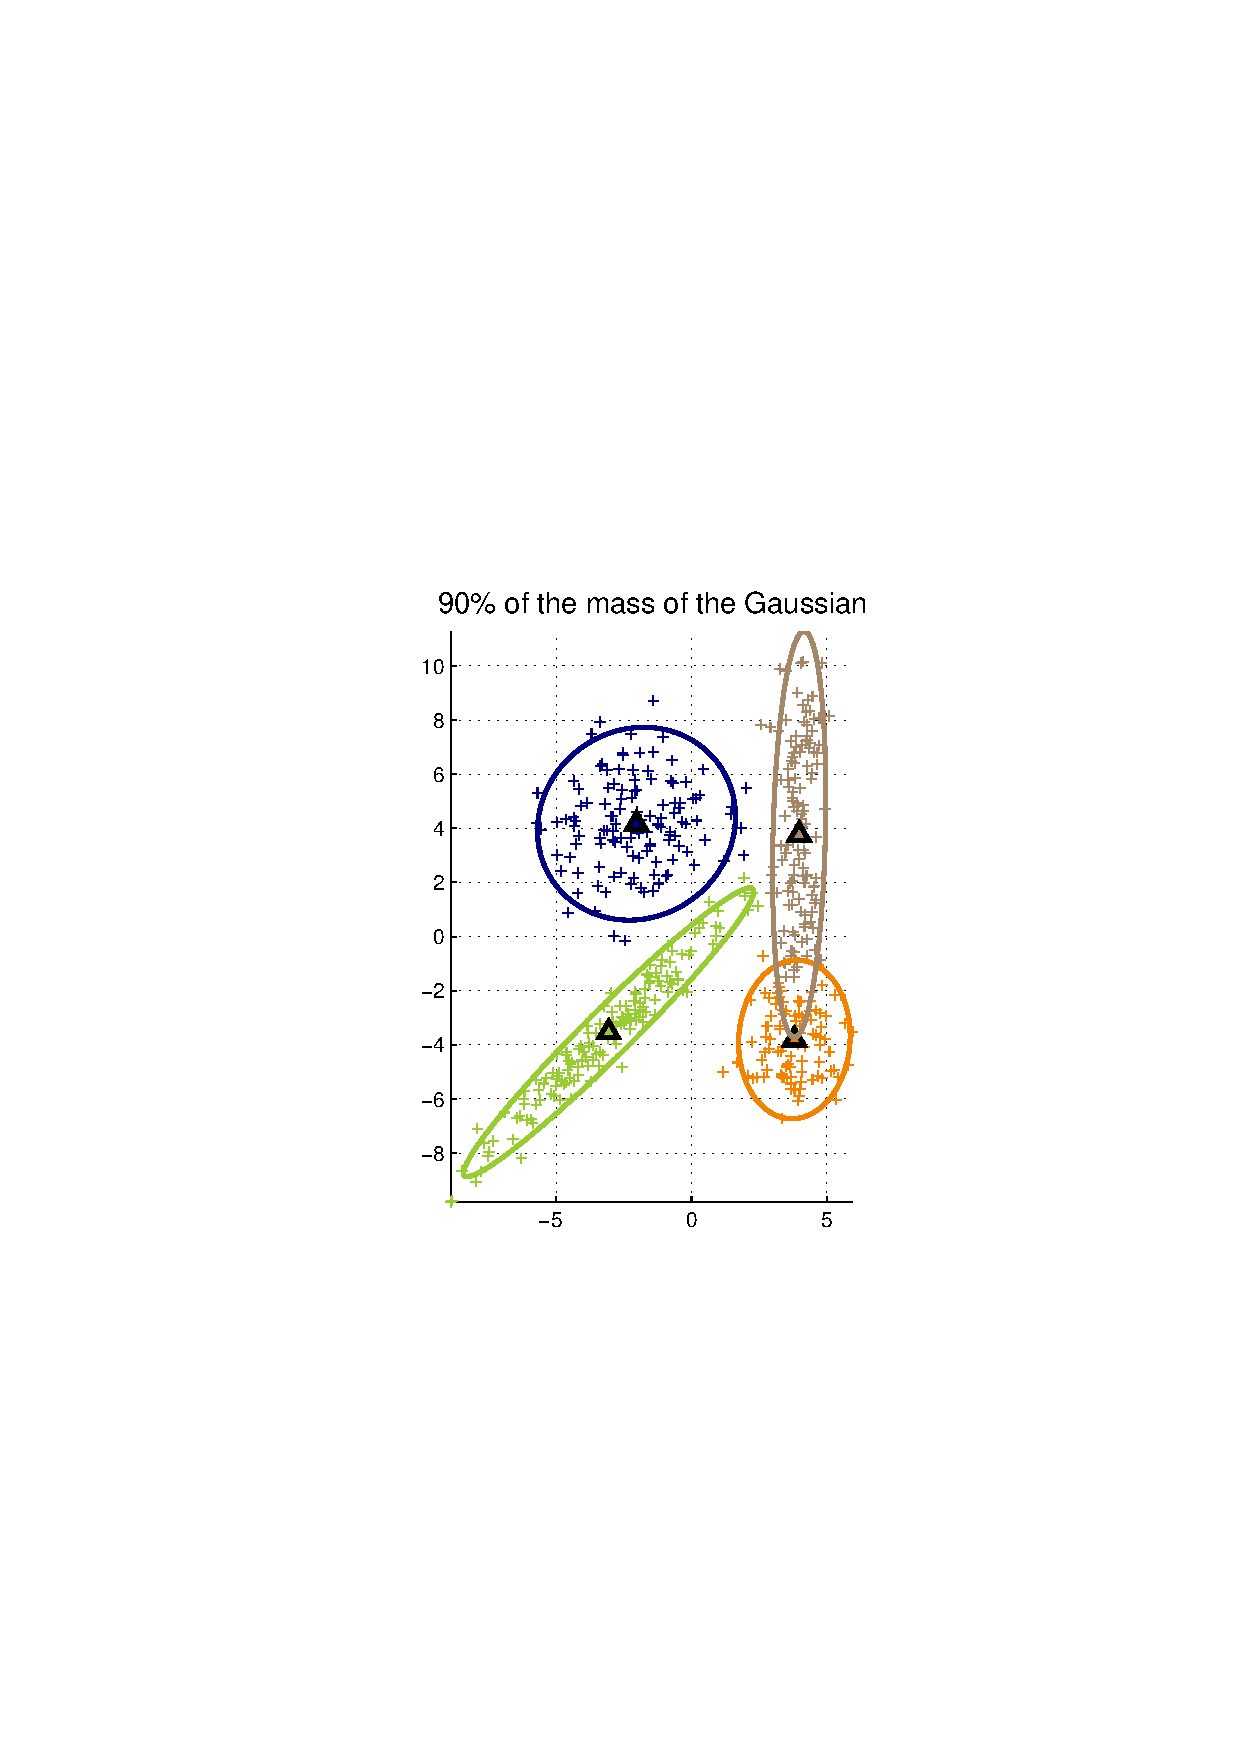
\includegraphics[width=.8\textwidth]{./pics/3c.pdf}
	\caption{Expectation maximization: 90\% mass of the Gaussian}
	\label{fig:3c}
\end{figure}

\subsection*{d}
\begin{figure} [H]
\centering
  \subfloat[Diagonal $\Sigma$]{\label{fig:3bTest} 
  		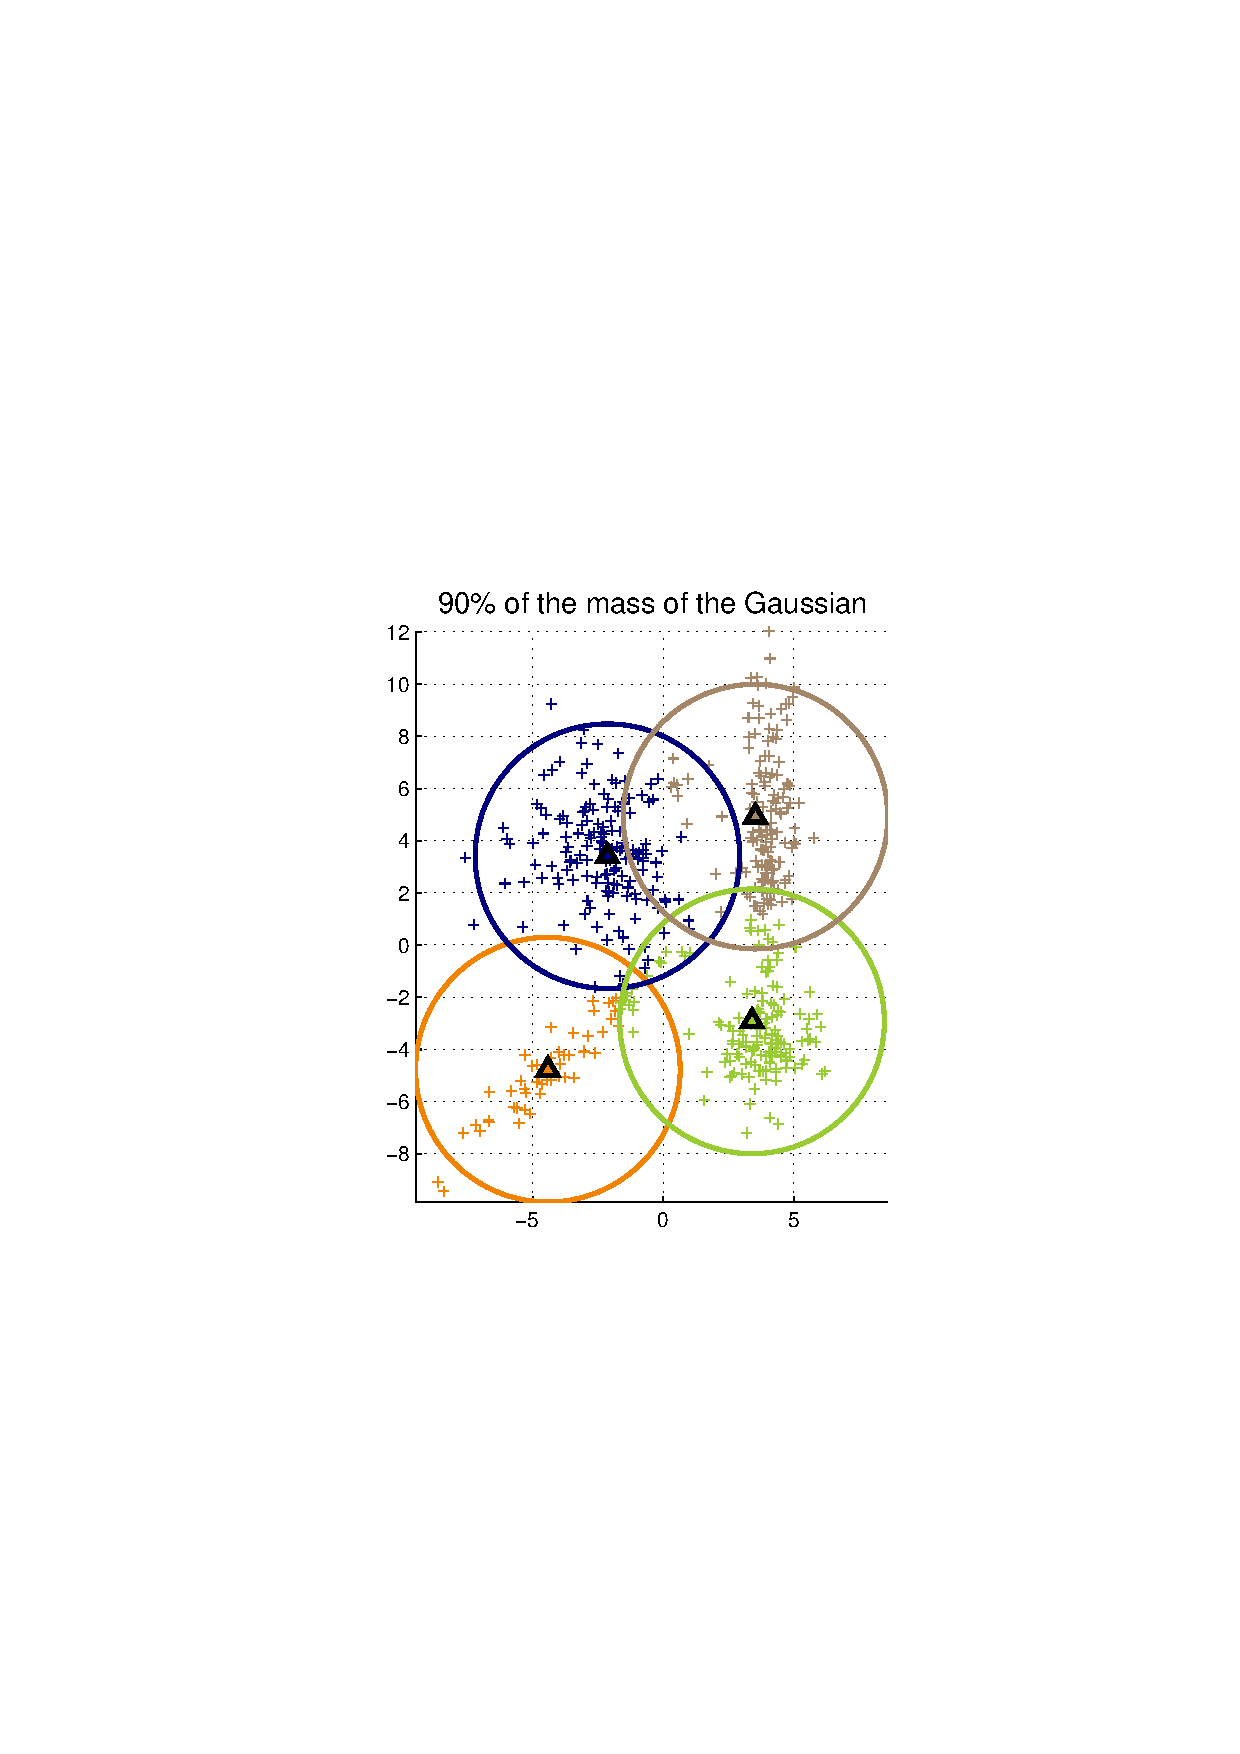
\includegraphics[width=.5\textwidth]{./pics/3bTest.pdf}} 
  \subfloat[General form $\Sigma$]{\label{fig:3cTest} 
  		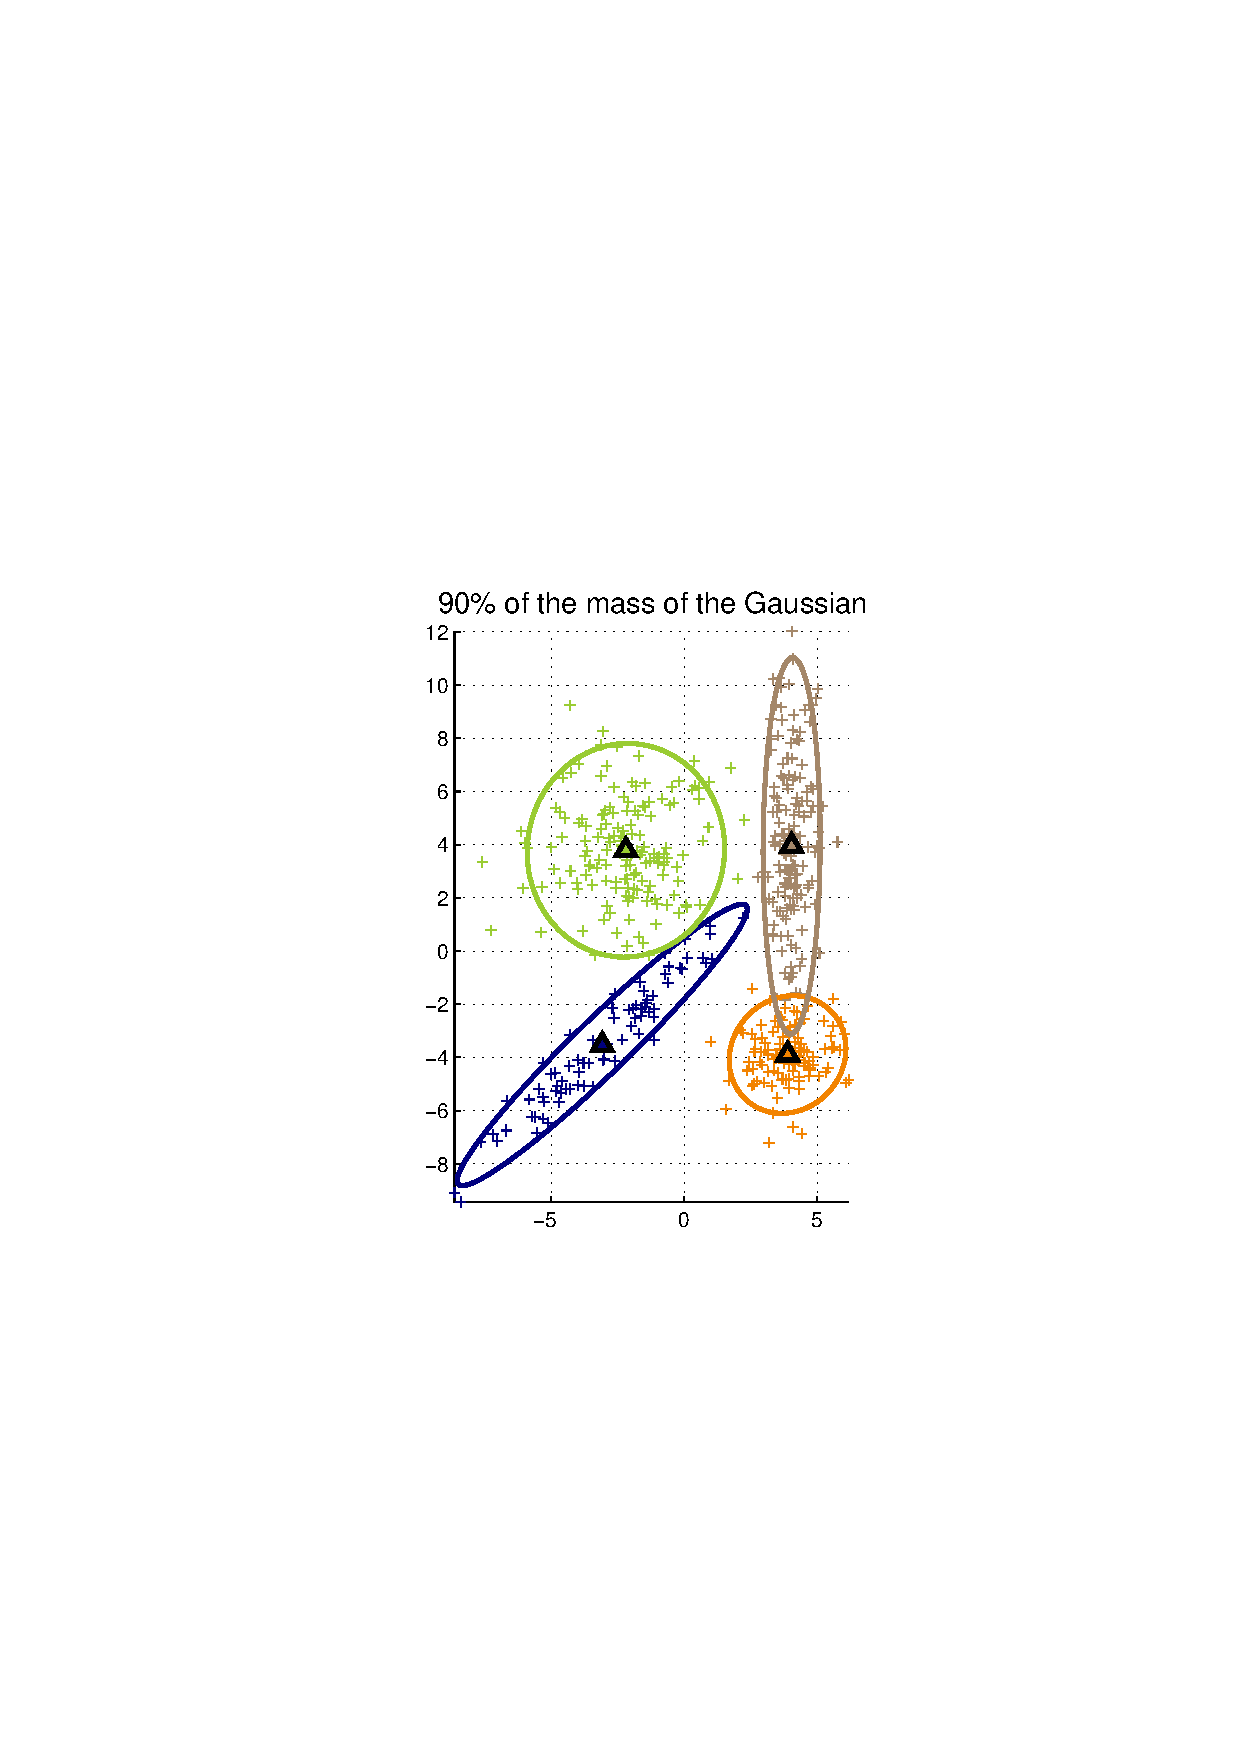
\includegraphics[width=.5\textwidth]{./pics/3cTest.pdf}} \\
  \caption{Results on test data} 
  \label{fig:3d}
\end{figure}

\begin{table}[H]
\centering
	\begin{tabular}{c|c|c|} 
	\cline{2-3}
	& \multicolumn{1}{c|}{\cellcolor[gray]{0.7} \textbf{Train}}  
	& \multicolumn{1}{c|}{\cellcolor[gray]{0.7} \textbf{Test}}
	\\ \hline
	
	\multicolumn{1}{|c|}{\cellcolor[gray]{0.8} \textbf{Diagonal Sigma}}   & -2843.4680 & -2798.0809 \\ \hline
	\multicolumn{1}{|c|}{\cellcolor[gray]{0.8} \textbf{General form Sigma}}   & -2370.8841
	 & -2399.2991 \\ \hline
	
	\end{tabular} 
	\caption{Final Likelihood}
	\label{tab:Likelihood}
\end{table}

>>>>>>> e9d7db917d331d85d092af225cf3a257f37b7431
\end{document}